% Graphic for TeX using PGF
% Title: /home/jannik/Dropbox/Projekte/Thesis/images/run_calibration.tex
% Creator: Dia v0.97.2
% CreationDate: Thu Mar  7 11:03:24 2013
% For: jannik
% \usepackage{tikz}
% The following commands are not supported in PSTricks at present
% We define them conditionally, so when they are implemented,
% this pgf file will use them.
\ifx\du\undefined
  \newlength{\du}
\fi
\setlength{\du}{15\unitlength}
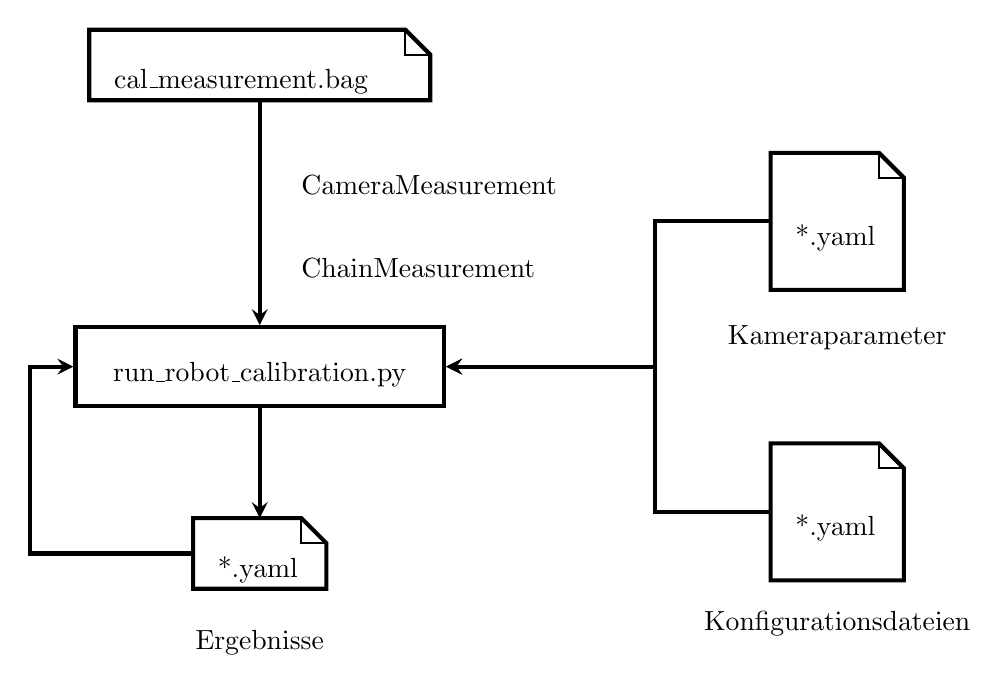
\begin{tikzpicture}
\pgftransformxscale{1.000000}
\pgftransformyscale{-1.000000}
\definecolor{dialinecolor}{rgb}{0.000000, 0.000000, 0.000000}
\pgfsetstrokecolor{dialinecolor}
\definecolor{dialinecolor}{rgb}{1.000000, 1.000000, 1.000000}
\pgfsetfillcolor{dialinecolor}
\pgfsetlinewidth{0.100000\du}
\pgfsetdash{}{0pt}
\definecolor{dialinecolor}{rgb}{1.000000, 1.000000, 1.000000}
\pgfsetfillcolor{dialinecolor}
\fill (9.002500\du,6.034870\du)--(16.617500\du,6.034870\du)--(17.217500\du,6.634870\du)--(17.217500\du,7.734870\du)--(9.002500\du,7.734870\du)--cycle;
\definecolor{dialinecolor}{rgb}{0.000000, 0.000000, 0.000000}
\pgfsetstrokecolor{dialinecolor}
\draw (9.002500\du,6.034870\du)--(16.617500\du,6.034870\du)--(17.217500\du,6.634870\du)--(17.217500\du,7.734870\du)--(9.002500\du,7.734870\du)--cycle;
\pgfsetlinewidth{0.050000\du}
\definecolor{dialinecolor}{rgb}{0.000000, 0.000000, 0.000000}
\pgfsetstrokecolor{dialinecolor}
\draw (16.617500\du,6.034870\du)--(16.617500\du,6.634870\du)--(17.217500\du,6.634870\du);
% setfont left to latex
\definecolor{dialinecolor}{rgb}{0.000000, 0.000000, 0.000000}
\pgfsetstrokecolor{dialinecolor}
\node[anchor=west] at (9.352500\du,7.279870\du){cal\_measurement.bag};
\definecolor{dialinecolor}{rgb}{1.000000, 1.000000, 1.000000}
\pgfsetfillcolor{dialinecolor}
\fill (8.670000\du,13.200000\du)--(8.670000\du,15.100000\du)--(17.550000\du,15.100000\du)--(17.550000\du,13.200000\du)--cycle;
\pgfsetlinewidth{0.100000\du}
\pgfsetdash{}{0pt}
\pgfsetdash{}{0pt}
\pgfsetmiterjoin
\definecolor{dialinecolor}{rgb}{0.000000, 0.000000, 0.000000}
\pgfsetstrokecolor{dialinecolor}
\draw (8.670000\du,13.200000\du)--(8.670000\du,15.100000\du)--(17.550000\du,15.100000\du)--(17.550000\du,13.200000\du)--cycle;
% setfont left to latex
\definecolor{dialinecolor}{rgb}{0.000000, 0.000000, 0.000000}
\pgfsetstrokecolor{dialinecolor}
\node at (13.110000\du,14.345000\du){run\_robot\_calibration.py};
% setfont left to latex
\definecolor{dialinecolor}{rgb}{0.000000, 0.000000, 0.000000}
\pgfsetstrokecolor{dialinecolor}
\node[anchor=west] at (13.110000\du,6.884870\du){};
\pgfsetlinewidth{0.100000\du}
\pgfsetdash{}{0pt}
\definecolor{dialinecolor}{rgb}{1.000000, 1.000000, 1.000000}
\pgfsetfillcolor{dialinecolor}
\fill (25.417657\du,16.000000\du)--(28.027657\du,16.000000\du)--(28.627657\du,16.600000\du)--(28.627657\du,19.300000\du)--(25.417657\du,19.300000\du)--cycle;
\definecolor{dialinecolor}{rgb}{0.000000, 0.000000, 0.000000}
\pgfsetstrokecolor{dialinecolor}
\draw (25.417657\du,16.000000\du)--(28.027657\du,16.000000\du)--(28.627657\du,16.600000\du)--(28.627657\du,19.300000\du)--(25.417657\du,19.300000\du)--cycle;
\pgfsetlinewidth{0.050000\du}
\definecolor{dialinecolor}{rgb}{0.000000, 0.000000, 0.000000}
\pgfsetstrokecolor{dialinecolor}
\draw (28.027657\du,16.000000\du)--(28.027657\du,16.600000\du)--(28.627657\du,16.600000\du);
% setfont left to latex
\definecolor{dialinecolor}{rgb}{0.000000, 0.000000, 0.000000}
\pgfsetstrokecolor{dialinecolor}
\node[anchor=west] at (25.767657\du,17.245000\du){};
% setfont left to latex
\definecolor{dialinecolor}{rgb}{0.000000, 0.000000, 0.000000}
\pgfsetstrokecolor{dialinecolor}
\node[anchor=west] at (25.767657\du,18.045000\du){*.yaml};
% setfont left to latex
\definecolor{dialinecolor}{rgb}{0.000000, 0.000000, 0.000000}
\pgfsetstrokecolor{dialinecolor}
\node[anchor=west] at (25.767657\du,18.845000\du){};
% setfont left to latex
\definecolor{dialinecolor}{rgb}{0.000000, 0.000000, 0.000000}
\pgfsetstrokecolor{dialinecolor}
\node at (27.022657\du,20.350000\du){Konfigurationsdateien};
\pgfsetlinewidth{0.100000\du}
\pgfsetdash{}{0pt}
\pgfsetdash{}{0pt}
\pgfsetmiterjoin
\pgfsetbuttcap
{
\definecolor{dialinecolor}{rgb}{0.000000, 0.000000, 0.000000}
\pgfsetfillcolor{dialinecolor}
% was here!!!
\pgfsetarrowsend{stealth}
{\pgfsetcornersarced{\pgfpoint{0.000000\du}{0.000000\du}}\definecolor{dialinecolor}{rgb}{0.000000, 0.000000, 0.000000}
\pgfsetstrokecolor{dialinecolor}
\draw (13.110000\du,7.781322\du)--(13.110000\du,9.000000\du)--(13.110000\du,9.000000\du)--(13.110000\du,13.151685\du);
}}
\pgfsetlinewidth{0.100000\du}
\pgfsetdash{}{0pt}
\pgfsetdash{}{0pt}
\pgfsetmiterjoin
\pgfsetbuttcap
{
\definecolor{dialinecolor}{rgb}{0.000000, 0.000000, 0.000000}
\pgfsetfillcolor{dialinecolor}
% was here!!!
\pgfsetarrowsend{stealth}
{\pgfsetcornersarced{\pgfpoint{0.000000\du}{0.000000\du}}\definecolor{dialinecolor}{rgb}{0.000000, 0.000000, 0.000000}
\pgfsetstrokecolor{dialinecolor}
\draw (25.367986\du,17.650000\du)--(22.628794\du,17.650000\du)--(22.628794\du,14.150000\du)--(17.600403\du,14.150000\du);
}}
% setfont left to latex
\definecolor{dialinecolor}{rgb}{0.000000, 0.000000, 0.000000}
\pgfsetstrokecolor{dialinecolor}
\node[anchor=west] at (13.838644\du,9.780789\du){CameraMeasurement};
% setfont left to latex
\definecolor{dialinecolor}{rgb}{0.000000, 0.000000, 0.000000}
\pgfsetstrokecolor{dialinecolor}
\node[anchor=west] at (13.838644\du,11.780789\du){ChainMeasurement};
\pgfsetlinewidth{0.100000\du}
\pgfsetdash{}{0pt}
\pgfsetdash{}{0pt}
\pgfsetmiterjoin
\pgfsetbuttcap
{
\definecolor{dialinecolor}{rgb}{0.000000, 0.000000, 0.000000}
\pgfsetfillcolor{dialinecolor}
% was here!!!
\pgfsetarrowsend{stealth}
{\pgfsetcornersarced{\pgfpoint{0.000000\du}{0.000000\du}}\definecolor{dialinecolor}{rgb}{0.000000, 0.000000, 0.000000}
\pgfsetstrokecolor{dialinecolor}
\draw (25.367986\du,10.650000\du)--(22.628794\du,10.650000\du)--(22.628794\du,14.150000\du)--(17.600403\du,14.150000\du);
}}
\pgfsetlinewidth{0.100000\du}
\pgfsetdash{}{0pt}
\definecolor{dialinecolor}{rgb}{1.000000, 1.000000, 1.000000}
\pgfsetfillcolor{dialinecolor}
\fill (25.417657\du,9.000000\du)--(28.027657\du,9.000000\du)--(28.627657\du,9.600000\du)--(28.627657\du,12.300000\du)--(25.417657\du,12.300000\du)--cycle;
\definecolor{dialinecolor}{rgb}{0.000000, 0.000000, 0.000000}
\pgfsetstrokecolor{dialinecolor}
\draw (25.417657\du,9.000000\du)--(28.027657\du,9.000000\du)--(28.627657\du,9.600000\du)--(28.627657\du,12.300000\du)--(25.417657\du,12.300000\du)--cycle;
\pgfsetlinewidth{0.050000\du}
\definecolor{dialinecolor}{rgb}{0.000000, 0.000000, 0.000000}
\pgfsetstrokecolor{dialinecolor}
\draw (28.027657\du,9.000000\du)--(28.027657\du,9.600000\du)--(28.627657\du,9.600000\du);
% setfont left to latex
\definecolor{dialinecolor}{rgb}{0.000000, 0.000000, 0.000000}
\pgfsetstrokecolor{dialinecolor}
\node[anchor=west] at (25.767657\du,10.245000\du){};
% setfont left to latex
\definecolor{dialinecolor}{rgb}{0.000000, 0.000000, 0.000000}
\pgfsetstrokecolor{dialinecolor}
\node[anchor=west] at (25.767657\du,11.045000\du){*.yaml};
% setfont left to latex
\definecolor{dialinecolor}{rgb}{0.000000, 0.000000, 0.000000}
\pgfsetstrokecolor{dialinecolor}
\node[anchor=west] at (25.767657\du,11.845000\du){};
% setfont left to latex
\definecolor{dialinecolor}{rgb}{0.000000, 0.000000, 0.000000}
\pgfsetstrokecolor{dialinecolor}
\node at (27.022657\du,13.454747\du){Kameraparameter};
\pgfsetlinewidth{0.100000\du}
\pgfsetdash{}{0pt}
\definecolor{dialinecolor}{rgb}{1.000000, 1.000000, 1.000000}
\pgfsetfillcolor{dialinecolor}
\fill (11.505000\du,17.800444\du)--(14.115000\du,17.800444\du)--(14.715000\du,18.400444\du)--(14.715000\du,19.500444\du)--(11.505000\du,19.500444\du)--cycle;
\definecolor{dialinecolor}{rgb}{0.000000, 0.000000, 0.000000}
\pgfsetstrokecolor{dialinecolor}
\draw (11.505000\du,17.800444\du)--(14.115000\du,17.800444\du)--(14.715000\du,18.400444\du)--(14.715000\du,19.500444\du)--(11.505000\du,19.500444\du)--cycle;
\pgfsetlinewidth{0.050000\du}
\definecolor{dialinecolor}{rgb}{0.000000, 0.000000, 0.000000}
\pgfsetstrokecolor{dialinecolor}
\draw (14.115000\du,17.800444\du)--(14.115000\du,18.400444\du)--(14.715000\du,18.400444\du);
% setfont left to latex
\definecolor{dialinecolor}{rgb}{0.000000, 0.000000, 0.000000}
\pgfsetstrokecolor{dialinecolor}
\node[anchor=west] at (11.855000\du,19.045444\du){*.yaml};
% setfont left to latex
\definecolor{dialinecolor}{rgb}{0.000000, 0.000000, 0.000000}
\pgfsetstrokecolor{dialinecolor}
\node at (13.110000\du,20.800444\du){Ergebnisse};
\pgfsetlinewidth{0.100000\du}
\pgfsetdash{}{0pt}
\pgfsetdash{}{0pt}
\pgfsetmiterjoin
\pgfsetbuttcap
{
\definecolor{dialinecolor}{rgb}{0.000000, 0.000000, 0.000000}
\pgfsetfillcolor{dialinecolor}
% was here!!!
\pgfsetarrowsend{stealth}
{\pgfsetcornersarced{\pgfpoint{0.000000\du}{0.000000\du}}\definecolor{dialinecolor}{rgb}{0.000000, 0.000000, 0.000000}
\pgfsetstrokecolor{dialinecolor}
\draw (13.110000\du,15.100000\du)--(13.110000\du,16.000000\du)--(13.110000\du,16.000000\du)--(13.110000\du,17.800444\du);
}}
\pgfsetlinewidth{0.100000\du}
\pgfsetdash{}{0pt}
\pgfsetdash{}{0pt}
\pgfsetmiterjoin
\pgfsetbuttcap
{
\definecolor{dialinecolor}{rgb}{0.000000, 0.000000, 0.000000}
\pgfsetfillcolor{dialinecolor}
% was here!!!
\pgfsetarrowsend{stealth}
{\pgfsetcornersarced{\pgfpoint{0.000000\du}{0.000000\du}}\definecolor{dialinecolor}{rgb}{0.000000, 0.000000, 0.000000}
\pgfsetstrokecolor{dialinecolor}
\draw (11.505000\du,18.650444\du)--(7.569726\du,18.650444\du)--(7.569726\du,14.150000\du)--(8.619726\du,14.150000\du);
}}
\end{tikzpicture}
